\documentclass[3p]{elsarticle}
\usepackage{ae,aecompl}
\usepackage[T1]{fontenc}
\usepackage[utf8]{inputenc}
\usepackage{pgfplots}
\usepackage{pst-plot}
\usepackage{tikz}
\usepgfplotslibrary{external}
\tikzexternalize
\usepackage{amsmath}
\usepackage{amssymb}
\usepackage{gensymb}
\usepackage{upgreek}
\usepackage{float}
\usepackage{indentfirst}
\parskip=0pt

\begin{document}

\begin{frontmatter}

\title{The effect of electric field on potentiometric Scanning Electrochemical Microscopic imaging}
\cortext[cor]{Corresponding author}
\author[akiss]{András Kiss\corref{cor}}
\address[akiss, gnagy]{Department of General and Physical Chemistry, Faculty of Sciences, University of Pécs, 7624 Pécs, Ifjúság útja 6, Hungary}
\address[rmsouto]{Department Chemistry, Universidad de La Laguna, P.O. Box 456, E-38200 La Laguna (Tenerife), Spain}
%\address[akiss, gnagy]{János Szentágothai Research Centre, University of Pécs, 7624 Pécs, Ifjúság Útja 20, Hungary}
\ead{akiss@gamma.ttk.pte.hu}
\author[dfilotas]{Dániel Filotás}
\ead{filotasdaniel@gmail.com}
\author[rmsouto]{Ricardo M. Souto}
\ead{rsouto@ull.es}
\author[gnagy]{Géza Nagy}
\ead{g-nagy@gamma.ttk.pte.hu}


\begin{abstract}

Potentiometric Scanning Electrochemical Microscopy (SECM) is a powerful tool in corrosion science.
It allows the selective imaging of a particular ionic species released at the anodic sites in a corrosion microcell, by using ion-selective microelectrodes (ISMEs) as scanning probes. Galvanic corrosion is a particularly often studied process.
The measured potential of the ISME is thought to depend only on the activity of the primary ion.
However, an electric field is also formed as a result of the potential difference between the surfaces of the galvanic pair, which has a direct influence on the potential of the sensing microelectrode; the measured potential is the sum of these two contributions.
The potential difference caused by the electric field can be substantially large, exceeding that of the potential difference associated with the activity of the primary ion.
In this paper, we present experimental evidence of this feature, and investigate the extent to which it influences the final chemically-resolved image. 
\end{abstract}
\begin{keyword}
	scanning electrochemical microscopy \sep potentiometry \sep ionselective microelectrode \sep galvanic corrosion \sep electric field
\end{keyword}
\end{frontmatter}

\section{Introduction}

In the past decade, potentiometric SECM -- sometimes referred to Scanning Ion Selective Electrode Technique (SIET) by the experts of this field -- has become increasingly popular among corrosion scientists \cite{lamaka, ZnISME, diamondel, cutedge, H+selective, simulating}.
The most extended application is the visualization of galvanic corrosion processes \cite{amperopot, chloride, spatiozn, fezn}.
Galvanic corrosion occurs when two dissimilar metals are both connected electrically and immersed in the same electrolyte. 
The electric coupling originates preferential and accelerated dissolution of the less noble metal acting as the anode of the corrosion cell, while the corrosion rate of the cathode is reduced.
The spatial separation of the anodic and the cathodic sites makes the complex corrosion processes readily interpretable, and due to the increased corrosion rates, conveniently shorter exposure times may be sufficient to obtain spatially-resolved images of the concentration distributions developed in the solution adjacent to the corroding sample.

Despite these beneficial circumstances, quantitative evaluation of galvanic corrosion using potentiometric SECM often fails due to –- up to now –- unrevealed reasons.
Izquierdo et al. reported discrepant results comparing Z-approach curves towards the cathode of a Mg-Fe galvanic couple obtained by either amperometric O$_2$ detection or potentiometric pH measurement \cite{pH15}. Local alkalinization could be detected even at 2 mm tip-substrate distance, whereas oxygen concentration already reached the bulk level at only ca. 900 $\upmu$m height. This discrepancy was attributed to an (unknown) contribution of the electric field to the potentiometric signal.  
In another works, the concentration of Mg$^{2+}$ that was detected using a Mg ISME above the Mg alloy disc, while galvanically coupled to iron, highly exceeded the upper limit of detection of the probe \cite{overmg1, overmg2, overmg3}.
On the other hand, pMg values fell below the lower limit of detection of Mg ISMEs scanning above cathodically polarized magnesium strips \cite{belowmg}. 

\begin{figure}
\centering
% trim = top left bottom right
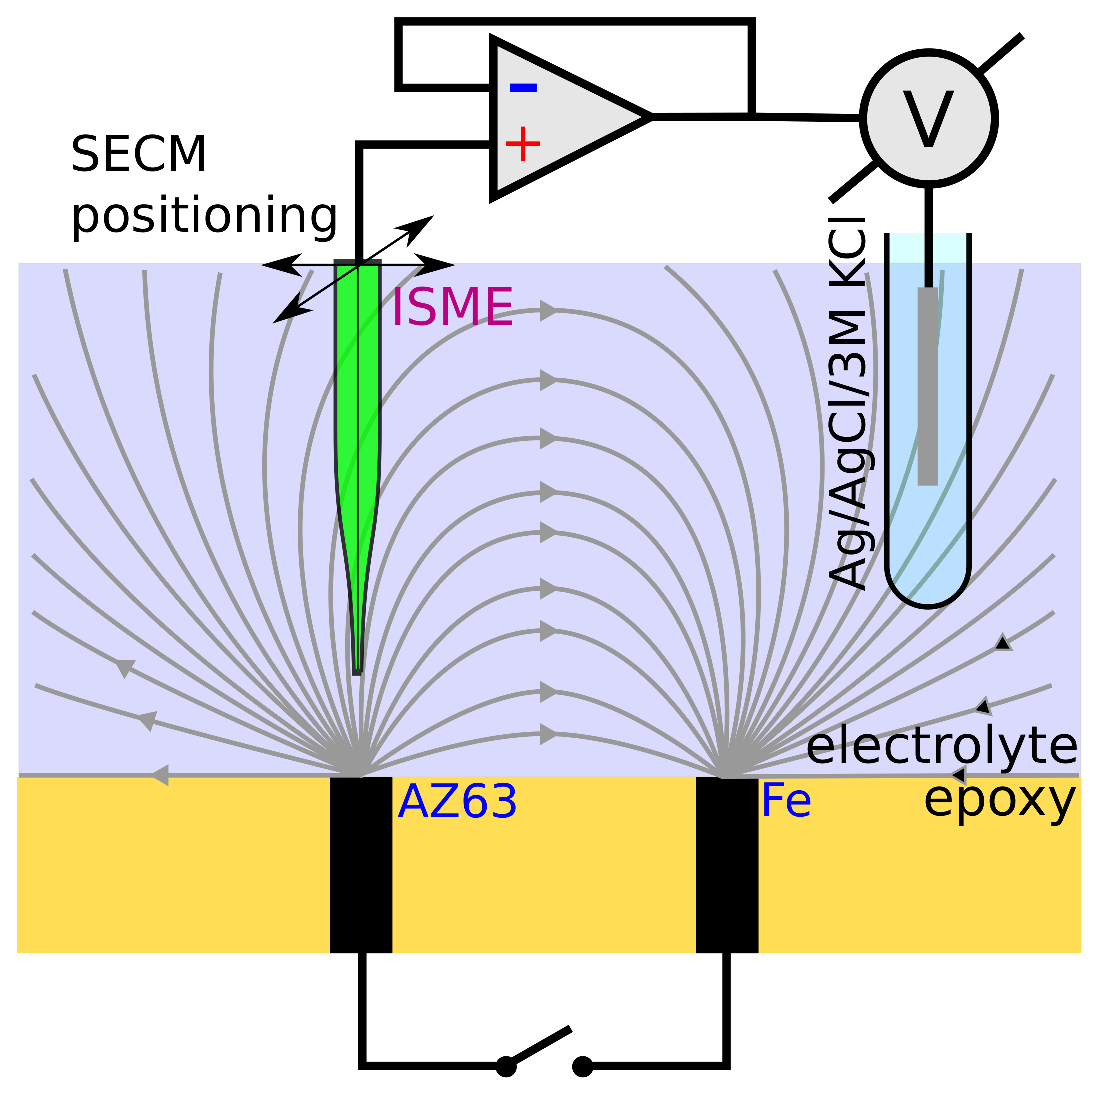
\includegraphics[width=0.5\textwidth]{abstract.eps}
\caption{An electric field is formed between the surfaces of the dissimilar metals constituting the galvanic couple. The potential difference between the measuring ($\phi_M$) and reference ($\phi_R$) electrodes is added to the Nernstian potential associated with the activity of the particular ion.}
\label{fig:abstract}
\end{figure}

These observations can be explained in terms of a contribution of the electric field to the measured potential. As it is well-known, the corrosion current is carried by electrons within the metallic phase, and it experiences negligible ohmic potential differences, because of the high conductivity of the material. Conversely, the ionic current flowing in the aqueous phase is associated with potential differences \cite{Isaacsfield}. 
That is, the potential difference between the anode and the cathode surfaces causes an electric field to be formed. 
This phenomenon is exploited in the Scanning Reference Electrode Technique (SRET), which allows to determine corrosion currents by actually measuring the potential variation in the solution with a scanning passive reference probe \cite{SRET1, SRET2, SRET3, SRET4}. 
The localized electric field SRET method has been progressively replaced by the more sensitive Scanning Vibrating Electrode Technique (SVET) in which a single vibrating probe is sensitive enough to detect smaller potential gradients arisen from ionic currents flowing in the solution \cite{SVET}. 
In the potentiometric SECM experiments cited above conducted on galvanic couples, the ISMEs must be subjected to the same effects. Then, as suspected by the above mentioned researchers, the local electric field may produce an undesired contribution to the potentiometric signal. 
The potential difference between the points where the electrodes are located is added to the potential difference associated with the primary ion activity at the tip of the measuring electrode (see fig. \ref{fig:abstract}):

\begin{equation}
\Delta E=E_M-E_R + (\phi_M - \phi_R)
\label{eq:potential}
\end{equation}

where $\Delta E$ is the measured potential difference, $E_R$ is the potential of the reference electrode, and $\phi_M$ and $\phi_R$ are the local potentials in the electric field at the measuring and reference electrodes, respectively. $E_M$ is the potential of the measuring ion-selective electrode for instance Mg$^{2+}$:

\begin{equation}
E_M = S \times lg[Mg^{2+}] + E_M^o
\label{eq:measuring}
\end{equation}

where $S$ is the slope of the calibration curve of the potentiometric cell with respect to the primary ion, and $E_M^o$ is the standard potential.
Since one could expect that the potential measured by the ISME is solely determined by the activity of the primary ions, and the aim of the experiments is to obtain quantitative and reliable concentration distributions of the species of interest, the additional contributions to the analytical signal have to be revealed.

In this contribution, the effect of the electric field on the measured potential difference at an ion-selective microelectrode probe has been investigated. The galvanic corrosion between an AZ63 Mg-Al alloy and iron was used as model system.

\section{Material and methods}

The preparation of solid contact Mg$^{2+}$ selective microelectrodes was described in detail before \cite{overmg3}. In brief, micropipettes were pulled from borosilicate capillaries (outer diameter $\oslash$ = 1.5 mm, inner dia. $\oslash$ = 1.0 mm, obtained from Hilgenberg GmbH, Malsfeld, Germany) with a Sutter Instruments P-30 type vertical capillary puller (Novato, CA, USA). The capillaries were silanized by 1 hour exposition to the saturated vapour of dichloro-dimethyl-silane at 120 $\celsius$. A poly-ethylen-dioxy-thiophene (PEDOT) coated carbon fiber of 33 $\upmu$m diameter (obtained as a generous gift from Specialty Materials, Lowell, MA, USA) served as the solid contact of the ISME. The PEDOT was electrochemically polymerized onto the carbon fiber and subsequently doped in KCl solution. The membrane components were purchased from Fluka (Buchs, Switzerland). The cocktail contains N,N''-Octamethylene-bis(N'-heptyl-N'-methyl-methylmalonamide inophore, 2-nitrophenyl-octyl ether emollient, PVC, potassium-[tetrakis-4-chlorophenyl]-borate and tetrahydrofuran. Eventually, the micropipette was front-filled with the cocktail, and the PEDOT-coated carbon fiber was inserted in the lumen of the capillary.
The Mg-ISMEs were calibrated by measuring their potential against an Ag/AgCl/KCl (3M) reference electrode in MgCl$_2$ solutions with tenfold increased concentrations between $10^{-7}$ and $10^{-1}$ M. The activities were calculated using the Debye-Hückel approach. A Nernstian relationship was observed between $10^{-1}$ and $10^{-5}$ M; the equation of the linear portion of the calibration curve is E = 29.5 mV/decade + 98.3 mV ($R^2=0.9997$). The lower limit of detection was pMg = 5.3.

The (Mg/Al)/Fe galvanic couple specimen was prepared using the AZ63 Mg/Al alloy and high purity Fe wires of 0.76 mm diameter. The wires were mounted in an epoxy resin sleeve (Struers, Ballerup, Denmark), exposing only the disk shaped surfaces at one side of the mould, and protruding at the rear side allowing to establish electric contact contact. Frontal surface of the mould was first ground with SiC paper up to 4000 grit, then polished with 1.0 and 0.3 $\upmu$m alumina powders.

SECM experiments were carried out using a homemade instrument operated with custom software. The potential values of the Mg ISMEs were measured respect to an Ag/AgCl (3M KCl) reference electrode. All the measurements were performed using a high input impedance eDAQ pH ISE isoPod USB (eDAQ Pty Ltd, Australia).

\section{Results and discussion}

A series of consecutive Z-approach curves were recorded above the corroding AZ63 sample (as shown in fig. \ref{fig:approach}A). The first 6 measurements were taken while the AZ63 sample was not electrically connected to the iron sample (red lines). As expected, Mg$^{2+}$ activity slowly increased with time as a result of spontaneous corrosion. The overall change was about 10 mV in 5 minutes. Next, the two metals were connected at the rear of the mould. As result of establishing the galvanic connection, there was an immediate rise of about 40 mV in the measured potential of the microelectrode (that is depicted by the transition from the red to the blue curves in fig. \ref{fig:approach}A). Since the galvanic coupling was established while the scanning tip was located 1000 $\upmu$m from the AZ63 sample, the reported change cannot possibly be attributed solely to an abrupt increase in Mg$^{2+}$ activity. Indeed, such a 40 mV change would correspond to an increase of ca. 1.5 orders of magnitude in Mg$^{2+}$ activity occuring in less than one second. Immediately after, six additional Z-approach curves were recorded during the galvanic coupling. The resulting accelerated dissolution of Mg$^{2+}$ can be distinguished from the blue curves in fig. \ref{fig:approach}A. Intense gas evolution could be observed on the surface of the AZ63 sample, which explains the noticeably more noisy curves recorded in this case. During this period of galvanic coupling, the potential sensed at the ISME, when situated at h = 1000 $\upmu$m, increased in app. 40 mV. This rise can be totally attributed to the increase in activity of the dissolving metal, i.e.: $\Delta E = 29.5 mV \times \Delta lg[$Mg$^{2+}]$. Finally, when the galvanic connection was stopped, 2 additional Z-approach curves were measured (green curves in fig. \ref{fig:approach}A). A sudden jump in potential (transition from blue to green curves) can be observed, of the same magnitude as before, though in the opposite direction, as a result of electric field vanishing. The shape of the latest Z-approach curves is very similar to the initial approaching curves recorded before galvanic connection was established, though they are shifted by about 40 mV in the positive direction. This is the result of the enhanced corrosion during the second phase of the experiment; Mg$^{2+}$ activity changed by about the same factor along the length of the scan-line. The shape of the Z-approach curves recorded during the galvanic coupling is notoriously different from those recorded during the spontaneous corrosion of the metal. This is because the contribution of the electric field, just like the contribution from Mg$^{2+}$, is not uniform at different distances on the scanned line. The strength of the electric field is inversely proportional to the square of the distance. The shape of the function 1/$z^2$ is recognizable from these plots.

\begin{figure}
\centering
\begin{tikzpicture}
\begin{axis}[ymin=-80, ymax=80, xmin=0, xmax=1000, xlabel={height, $\upmu$m}, ylabel={E, mV vs Ag/AgCl/ 3M KCl}, clip marker paths=true, width=7cm, height=7cm, legend style={draw=none}, legend cell align=left]
\addplot [domain=0:1000, color=red, y filter/.code={\pgfmathparse{\pgfmathresult*1000}}] table {1.txt};
\addplot [domain=0:1000, color=red, y filter/.code={\pgfmathparse{\pgfmathresult*1000}}] table {2.txt};
\addplot [domain=0:1000, color=red, y filter/.code={\pgfmathparse{\pgfmathresult*1000}}] table {3.txt};
\addplot [domain=0:1000, color=red, y filter/.code={\pgfmathparse{\pgfmathresult*1000}}] table {4.txt};
\addplot [domain=0:1000, color=red, y filter/.code={\pgfmathparse{\pgfmathresult*1000}}] table {5.txt};
\addplot [domain=0:1000, color=red, y filter/.code={\pgfmathparse{\pgfmathresult*1000}}] table {6.txt};
\addplot [domain=0:1000, color=red, y filter/.code={\pgfmathparse{\pgfmathresult*1000}}] table {7.txt};
\addplot [domain=0:1000, color=blue, dashed, y filter/.code={\pgfmathparse{\pgfmathresult*1000}}] table {8.txt};
\addplot [domain=0:1000, color=blue, dashed, y filter/.code={\pgfmathparse{\pgfmathresult*1000}}] table {9.txt};
\addplot [domain=0:1000, color=blue, dashed, y filter/.code={\pgfmathparse{\pgfmathresult*1000}}] table {10.txt};
\addplot [domain=0:1000, color=blue, dashed, y filter/.code={\pgfmathparse{\pgfmathresult*1000}}] table {11.txt};
\addplot [domain=0:1000, color=blue, dashed, y filter/.code={\pgfmathparse{\pgfmathresult*1000}}] table {12.txt};
\addplot [domain=0:1000, color=blue, dashed, y filter/.code={\pgfmathparse{\pgfmathresult*1000}}] table {13.txt};
\addplot [domain=0:1000, color=green, densely dashdotted, y filter/.code={\pgfmathparse{\pgfmathresult*1000}}] table {14.txt};
\addplot [domain=0:1000, color=green, densely dashdotted, y filter/.code={\pgfmathparse{\pgfmathresult*1000}}] table {15.txt};
\node[anchor=north east] at (rel axis cs:0.98,0.98) {A};

%\draw [black, ->] (axis cs:900,-0.05) -- (axis cs:900,-0.025);
%\node[black, left] at (axis cs:900,-0.0375) {$\Delta$E$_1$};


%\node[black, above left] at (axis cs:0,-290) {pH 4};
%\node[black, above right] at (axis cs:0,-290) {pH 6};
%\addplot +[mark=none] coordinates {(0, -300)-.- (0, -100)};
%\draw [dashed, black] (axis cs:0,-300) -- (axis cs:0,-100);
%\addlegendentry{raw recording}
%\addlegendentry{$E = - 280 + 97 e^{-t/3.76}$}
%\addlegendentry{$E = - 280 + 97 (e^{-t/9} + e^{-t/0.5577})/2$}
\end{axis}
\end{tikzpicture}
\begin{tikzpicture}
\begin{axis}[ymin=-75, ymax=200, xmin=0, xmax=680, xlabel={time, s}, ylabel={E, mV vs Ag/AgCl/ 3M KCl}, clip marker paths=true, width=7cm, height=7cm, legend style={draw=none}, legend cell align=left]
\addplot [domain=-30:100, color=red, mark=*] table {on_off_100.txt};
\addplot [domain=-30:100, color=blue, mark=*] table {on_off_1000.txt};
\node[anchor=north east] at (rel axis cs:0.98,0.98) {B};

\node[red, above right] at (axis cs:40,20) {h = 100 $\upmu$m};
\node[blue, above right] at (axis cs:40,-50) {h = 1000 $\upmu$m};
%\addplot +[mark=none] coordinates {(0, -300)-.- (0, -100)};
\draw [black, ->] (axis cs:320,125) -- (axis cs:320,100);
\node[black, above] at (axis cs:320,125) {on};
\draw [black, ->] (axis cs:460,125) -- (axis cs:460,100);
\node[black, above] at (axis cs:460,125) {off};

%\addlegendentry{raw recording}
%\addlegendentry{$E = - 280 + 97 e^{-t/3.76}$}
%\addlegendentry{$E = - 280 + 97 (e^{-t/9} + e^{-t/0.5577})/2$}
\end{axis}
\end{tikzpicture}
\caption{(A) Sequence of consecutive Z-approach curves recorded above the center of the AZ63 wire with a Mg$^{2+}$ ISME. Step size: 10 $\upmu$m. 500 ms settling time was allowed for the potentiometric cell at each points before measurements. Lines in chronological order: solid red = spontaneous corrosion, dashed blue = galvanic corrosion, dash dotted green = spontaneous corrosion. (B) Stationary recordings above the center of the AZ63 target with the ISME placed at: red = 100 $\upmu$m, blue = 1000 $\upmu$m distance from the metal. On/off denote the moment when galvanic coupling was either established or ceased. Temporal resolution was 1 Hz.}
\label{fig:approach}
\end{figure}



In another series of experiments, the ISME was maintained at a constant height from the metal surface, and its potential was recorded as a function of time, while the galvanic connection was established between the two metals by the operator (fig. \ref{fig:approach}B). Thus, the tip was first positioned 100 $\upmu$m above the center of the AZ63 wire (red curve in fig. \ref{fig:approach}B), and for about 300 s the spontaneous corrosion of the alloy sample was recorded. Then, the galvanic connection was established, and a sharp increase in potential of about 70 mV could be observed. This change would correspond to a two orders of magnitude increase of Mg$^{2+}$ activity in a very short period of time. When the galvanic connection was removed, a potential change of the same magnitude, though opposite direction could be observed. In order to discard the possibility that this rise could be still explained by an abrupt release of Mg$^{2+}$ from the surface, the experiment was repeated while the tip was positioned 1000 $\upmu$m above the target (blue curve in fig. \ref{fig:approach}B). A very similar sequence of potential changes could be observed, despite the big separation between the probe and the corroding sample. Even if one argues a change in Mg$^{2+}$ activity of more than two orders of magnitude is possible 100 $\upmu$m away the source in less than a second, it cannot be the case 1000 $\upmu$m from it. The only plausible explanation is that the abrupt change in the recorded potential is due to the electric field developed between the two metals. 

Finally, in order to demonstrate the influence of the electric field on SECM imaging, measurements were made after 30 minutes of galvanic coupling by using a constant 100 $\upmu$m tip-sample distance. 
Then the galvanic connection was ceased, and immediately another 2D scan was recorded above the Mg disk. The sequence of the two images can be seen in fig. \ref{fig:2d}. Apparently, in the case of galvanic coupling, a 0.1 M Mg$^{2+}$ activity is monitored even in the bulk of the solution, whereas above the center of the disk the activity reaches the implausible 10$^{4}$ M value by using the calibration curve for calculation.   
In fig. \ref{fig:2d}B the measured values are in the linear range of the ISME, and the overall potential change is several orders of magnitude smaller than in fig. \ref{fig:2d}A.


\def\s{0.35}
\begin{figure}
\centering
% trim = top left bottom right
\includegraphics[trim = 10mm 20mm 0mm 10mm, clip, width=\s\textwidth, angle=-90]{17012501.eps}\includegraphics[trim = 10mm 20mm 0mm 10mm, clip, width=\s\textwidth, angle=-90]{17012503_deconvoluted.eps}
\caption{2D Mg$^{2+}$ ion distributions above the AZ63 wire while: (A) galvanically connected to Fe and (B) immediately after ceasing electrical connection between the two metallic materials. Tip-sample distance: 100 $\upmu$m.}
\label{fig:2d}
\end{figure}





\section{Conclusions}

The effect of the electric field in certain potentiometric SECM experiments has been demonstrated experimentally, as suspected by certain researchers in corrosion science for some time. A strong electric field is formed around galvanic coupling of dissimilar metals, that causes significant over- or underestimations of the real primary ion activity. The reason for this feature is that the electric field has a direct influence on the measured potential at the ISME.

Based on the findings described in this work, this effect should be minimised by bringing the reference and measuring electrodes very close together, so the electric field experienced by the two components is equal, and therefore it cancels out. An alternative solution might involve to operate an electric relay as a switch between the galvanic couple, and disconnect them for a very short period of time, while the measurement is performed. These two possible solutions will be subject of further investigation in our research groups.

%\section{Acknowledgements}
%The authors would like to thank Dr. Sándor Kunsági-Máté the discussion about the electric field.

\section*{References}

\begin{thebibliography}{5}

\bibitem{lamaka}S.V. Lamaka, M.G. Taryba, M.L. Zheludkevich, M.G.S. Ferreira, Novel solid-contact ion-selective microelectrodes for localized potentiometric measurements, Electroanalysis 21 (2009) 2447-2453.
\bibitem{ZnISME}J. Izquierdo, L. Nagy, Á. Varga, I. Bitter, G. Nagy, R.M. Souto, Scanning electrochemical microscopy for the investigation of corrosion processes: Measurement of  $Zn^{2+}$ spatial distribution with ion selective microelectrodes, Electrochimica Acta 59 (2012) 398–403. 
\bibitem{diamondel}E.L. Silva, A.C. Bastos, M.A. Neto, R.F. Silva, M.G.S. Ferreira, M.L. Zheludkevich, F.J. Oliveira, Novel diamond microelectrode for pH sensing, Electrochemistry Communications 40 (2014) 31–34.
\bibitem{cutedge}A. Alvarez-Pampliega, S.V. Lamaka, M.G. Taryba, M. Madani, J. De Strycker, E. Tourwé, M.G.S. Ferreira, H. Terryn, Cut-edge corrosion study on painted aluminum rich metallic coated steel by scanning vibrating electrode and micro-potentiometric techniques Electrochimica Acta 61 (2012) 107–117.	
\bibitem{H+selective}E.A. Zdrachek. A.G. Karotkaya, V.A. Nazarov, K.A. Andronchyk, L.S. Stanishevskii, V.V. Egorov, M.G. Taryba, D. Snihirova, M. Kopylovich, S.V. Lamaka $H^{+}$-selective microelectrodes with optimized measuring range for corrosion studies, Sensors and Actuators B 207 (2015) 967–975.
\bibitem{simulating}H. Shi, Z. Tian, T. Hu, F. Liu, E. H. Han, M. Taryba, S.V. Lamaka Simulating corrosion of Al$_{2}$CuMg phase by measuring ionic currents, chloride concentration and pH, Corrosion Science 88 (2014) 178–186.
\bibitem{amperopot}J. Izquierdo, L. Nagy, J.J. Santana, G. Nagy, R.M. Souto, A novel microelectrochemical strategy for the study of corrosion inhibitors employing the scanning vibrating electrode technique and dual potentiometric/amperometric operation in scanning electrochemical microscopy: Application to the study of the cathodic inhibition by benzotriazole of the galvanic corrosion of copper coupled to iron, Electrochimica Acta 58 (2011) 707-716.
\bibitem{chloride}V.A. Nazarov, M.G. Taryba, E.A. Zdrachek, K.A. Andronchyk, V.V. Egorov, S.V. Lamaka, Sodium- and chloride-selective microelectrodes optimized for corrosion studies, Journal of Electroanalytical Chemistry 706 (2013) 13–24.
\bibitem{spatiozn}E. Tada, S. Satoh, H. Kaneko,The spatial distribution of $Zn^{2+}$ during galvanic corrosion of a Zn/steel couple, Electrochimica Acta 49 (2004) 2279–2285.
\bibitem{fezn}A.G. Marques M. Taryba A.S. Panao S. Lamaka, A.M. Simoes, Application of scanning electrode techniques for the evaluation of iron–zinc corrosion in nearly neutral chloride solutions, Corrosion Science 104 (2016) 123-131.
\bibitem{pH15}J. Izquierdo, L. Nagy, I. Bitter, R.M. Souto, G. Nagy, 
Potentiometric scanning electrochemical microscopy for the local characterization of the electrochemical behaviour of magnesium-based materials, Electrochimica Acta 87 (2013) 283–293.
\bibitem{overmg1}R.M. Souto, A. Kiss, J. Izquierdo, L. Nagy, I. Bitter, G. Nagy, Spatially-resolved imaging of concentration distributions on corroding magnesium-based materials exposed to aqueous environments by SECM, Electrochemistry Communications 26 (2013) 25–28.
\bibitem{overmg2}R.M. Souto, J Izquierdo, J.J. Santana, A Kiss, L Nagy, G Nagy 
Progress in scanning electrochemical microscopy by coupling potentiometric and amperometric measurement modes
A Méndez-Vilas (Ed.)
Current microscopy contributions to advances in science and technology. Formatex Research Center, Badajoz Spain 2012. pp. 1407-1415.
\bibitem{overmg3}J. Izquierdo, A. Kiss, J. J. Santana, L. Nagy, I. Bitter, H. S. Isaacs, G. Nagy, R. M. Souto
Development of $Mg^{2+}$ ion-selective microelectrodes for potentiometric scanning electrochemical microscopy monitoring of galvanic corrosion processes
Journal of the Electrochemical Society  160 (2013) 451-459. 
\bibitem{belowmg}J. Izquierdo, B. M. Fernández-Pérez, D. Filotás, Z. Őri, A. Kiss, R.T. Martín-Gómez, L. Nagy, G. Nagy, R. M. Souto, Imaging of concentration distributions and hydrogen evolution on corroding magnesium exposed to aqueous environments using scanning electrochemical microscopy, Electroanalysis 28 (2016) 1–14.
\bibitem{Isaacsfield}H.S. Isaacs, B. Vyas Scanning reference electrode techniques in localized corrosion, in: F. Mansfeld, U. Bertocci (Eds.), Electrochemical Corrosion Testing, ASTM STP 727, American Society for Testing and Materials, Philadelphia PA, 1981, p. 31.
\bibitem{SRET1}H.N. McMurray, S.R. Magill, B.D. Jeffs, Scanning reference electrode technique as tool for investigating localised corrosion phenomena in galvanised steels, Ironmaking \& Steelmaking 23 (1996) 183–188.
\bibitem{SRET2}V.S. Voruganti, H.B. Luft, D. DeGeer, S.A. Bradford, Scanning reference electrode technique for the investigation of preferential corrosion of weldments in offshore applications, Corrosion 47 (1991) 343–351.
\bibitem{SRET3}H.S. Isaacs, G. Kissel, Surface preparation and pit propagation in stainless steels, Journal of The Electrochemical Society 119 (1972) 1628–1632.
\bibitem{SRET4}N. Hsu, J.D. Garber, R. Brunel, R.D. Braun, A scanning reference electrode for use during corrosive measurements, Corrosion 43 (1987) 606–610.
\bibitem{SVET}H.S. Isaacs, The use of the scanning vibrating electrode technique for detecting defects in ion vapor-deposited aluminum on steel, Corrosion 43 (1987) 594–598.   


\end{thebibliography}

\end{document}
